% Options for packages loaded elsewhere
\PassOptionsToPackage{unicode}{hyperref}
\PassOptionsToPackage{hyphens}{url}
%
\documentclass[
]{article}
\usepackage{amsmath,amssymb}
\usepackage{iftex}
\ifPDFTeX
  \usepackage[T1]{fontenc}
  \usepackage[utf8]{inputenc}
  \usepackage{textcomp} % provide euro and other symbols
\else % if luatex or xetex
  \usepackage{unicode-math} % this also loads fontspec
  \defaultfontfeatures{Scale=MatchLowercase}
  \defaultfontfeatures[\rmfamily]{Ligatures=TeX,Scale=1}
\fi
\usepackage{lmodern}
\ifPDFTeX\else
  % xetex/luatex font selection
\fi
% Use upquote if available, for straight quotes in verbatim environments
\IfFileExists{upquote.sty}{\usepackage{upquote}}{}
\IfFileExists{microtype.sty}{% use microtype if available
  \usepackage[]{microtype}
  \UseMicrotypeSet[protrusion]{basicmath} % disable protrusion for tt fonts
}{}
\makeatletter
\@ifundefined{KOMAClassName}{% if non-KOMA class
  \IfFileExists{parskip.sty}{%
    \usepackage{parskip}
  }{% else
    \setlength{\parindent}{0pt}
    \setlength{\parskip}{6pt plus 2pt minus 1pt}}
}{% if KOMA class
  \KOMAoptions{parskip=half}}
\makeatother
\usepackage{xcolor}
\usepackage[margin=1in]{geometry}
\usepackage{graphicx}
\makeatletter
\def\maxwidth{\ifdim\Gin@nat@width>\linewidth\linewidth\else\Gin@nat@width\fi}
\def\maxheight{\ifdim\Gin@nat@height>\textheight\textheight\else\Gin@nat@height\fi}
\makeatother
% Scale images if necessary, so that they will not overflow the page
% margins by default, and it is still possible to overwrite the defaults
% using explicit options in \includegraphics[width, height, ...]{}
\setkeys{Gin}{width=\maxwidth,height=\maxheight,keepaspectratio}
% Set default figure placement to htbp
\makeatletter
\def\fps@figure{htbp}
\makeatother
\setlength{\emergencystretch}{3em} % prevent overfull lines
\providecommand{\tightlist}{%
  \setlength{\itemsep}{0pt}\setlength{\parskip}{0pt}}
\setcounter{secnumdepth}{-\maxdimen} % remove section numbering
\usepackage{booktabs}
\usepackage{longtable}
\usepackage{array}
\usepackage{multirow}
\usepackage{wrapfig}
\usepackage{float}
\usepackage{colortbl}
\usepackage{pdflscape}
\usepackage{tabu}
\usepackage{threeparttable}
\usepackage{threeparttablex}
\usepackage[normalem]{ulem}
\usepackage{makecell}
\usepackage{xcolor}
\ifLuaTeX
  \usepackage{selnolig}  % disable illegal ligatures
\fi
\usepackage{bookmark}
\IfFileExists{xurl.sty}{\usepackage{xurl}}{} % add URL line breaks if available
\urlstyle{same}
\hypersetup{
  pdftitle={Arbitrary Experiment},
  hidelinks,
  pdfcreator={LaTeX via pandoc}}

\title{Arbitrary Experiment}
\author{}
\date{\vspace{-2.5em}}

\begin{document}
\maketitle

\section{Analyze attack trends}\label{analyze-attack-trends}

\begingroup\fontsize{9}{11}\selectfont

\begin{longtable}[t]{llllrrrrrr}
\caption{\label{tab:arbitrary_trend_table}We run a logistic model regressing success against perturb-target distance and perturb box length, both relative to image width or height, in the deliberate attack experiment. Longer perturb box length or shorter perturb-target distance cause success rates to significantly increase for all model and attack combinations, except for perturb box length in untargeted attack on Cascade R-CNN. The interaction terms, even when significant, are negligibly close to 0. Table headers are explained in Appendix \ref{app:tab_hdr}.}\\
\toprule
\multicolumn{2}{c}{Group} & \multicolumn{8}{c}{Regression} \\
\cmidrule(l{3pt}r{3pt}){1-2} \cmidrule(l{3pt}r{3pt}){3-10}
 & Attack & term & sig & estimate & std.error & statistic & p.value & conf.low & conf.high\\
\midrule
\addlinespace[0.3em]
\multicolumn{10}{l}{\textbf{YOLOv3}}\\
\hspace{1em} & Vanishing & distance & * & -6.047 & 1.227 & -4.928 & 0.000 & -8.472 & -3.660\\
\cmidrule{3-10}\nopagebreak
\hspace{1em} &  & length & * & 8.243 & 0.530 & 15.558 & 0.000 & 7.227 & 9.305\\
\cmidrule{3-10}\nopagebreak
\hspace{1em} &  & distance * length & * & -18.211 & 3.543 & -5.140 & 0.000 & -25.189 & -11.292\\
\cmidrule{2-10}\nopagebreak
\hspace{1em} & Mislabeling & distance & * & -7.151 & 1.231 & -5.810 & 0.000 & -9.588 & -4.761\\
\cmidrule{3-10}\nopagebreak
\hspace{1em} &  & length & * & 5.888 & 0.395 & 14.922 & 0.000 & 5.126 & 6.674\\
\cmidrule{3-10}\nopagebreak
\hspace{1em} &  & distance * length &  & -3.239 & 3.100 & -1.045 & 0.296 & -9.296 & 2.862\\
\cmidrule{2-10}\nopagebreak
\hspace{1em} & Untargeted & distance & * & -9.320 & 1.515 & -6.153 & 0.000 & -12.343 & -6.401\\
\cmidrule{3-10}\nopagebreak
\hspace{1em} &  & length & * & 2.063 & 0.285 & 7.245 & 0.000 & 1.508 & 2.624\\
\cmidrule{3-10}\nopagebreak
\hspace{1em} &  & distance * length &  & 4.340 & 2.943 & 1.475 & 0.140 & -1.392 & 10.150\\
\cmidrule{1-10}\pagebreak[0]
\addlinespace[0.3em]
\multicolumn{10}{l}{\textbf{SSD}}\\
\hspace{1em} & Vanishing & distance & * & -10.417 & 1.552 & -6.711 & 0.000 & -13.513 & -7.424\\
\cmidrule{3-10}\nopagebreak
\hspace{1em} &  & length & * & 4.737 & 0.318 & 14.882 & 0.000 & 4.120 & 5.368\\
\cmidrule{3-10}\nopagebreak
\hspace{1em} &  & distance * length &  & -3.353 & 3.072 & -1.091 & 0.275 & -9.345 & 2.705\\
\cmidrule{2-10}\nopagebreak
\hspace{1em} & Mislabeling & distance & * & -7.996 & 1.697 & -4.712 & 0.000 & -11.385 & -4.729\\
\cmidrule{3-10}\nopagebreak
\hspace{1em} &  & length & * & 6.065 & 0.345 & 17.570 & 0.000 & 5.397 & 6.750\\
\cmidrule{3-10}\nopagebreak
\hspace{1em} &  & distance * length & * & -12.651 & 3.354 & -3.772 & 0.000 & -19.201 & -6.047\\
\cmidrule{2-10}\nopagebreak
\hspace{1em} & Untargeted & distance & * & -9.777 & 1.868 & -5.233 & 0.000 & -13.530 & -6.201\\
\cmidrule{3-10}\nopagebreak
\hspace{1em} &  & length & * & 3.798 & 0.314 & 12.094 & 0.000 & 3.188 & 4.419\\
\cmidrule{3-10}\nopagebreak
\hspace{1em} &  & distance * length & * & -7.443 & 3.635 & -2.048 & 0.041 & -14.527 & -0.268\\
\cmidrule{1-10}\pagebreak[0]
\addlinespace[0.3em]
\multicolumn{10}{l}{\textbf{RetinaNet}}\\
\hspace{1em} & Vanishing & distance & * & -23.008 & 3.077 & -7.477 & 0.000 & -29.253 & -17.194\\
\cmidrule{3-10}\nopagebreak
\hspace{1em} &  & length & * & 2.583 & 0.345 & 7.491 & 0.000 & 1.912 & 3.264\\
\cmidrule{3-10}\nopagebreak
\hspace{1em} &  & distance * length &  & -10.769 & 6.353 & -1.695 & 0.090 & -23.153 & 1.757\\
\cmidrule{2-10}\nopagebreak
\hspace{1em} & Mislabeling & distance & * & -22.522 & 4.237 & -5.316 & 0.000 & -31.273 & -14.667\\
\cmidrule{3-10}\nopagebreak
\hspace{1em} &  & length & * & 1.261 & 0.419 & 3.007 & 0.003 & 0.443 & 2.087\\
\cmidrule{3-10}\nopagebreak
\hspace{1em} &  & distance * length &  & 1.459 & 8.334 & 0.175 & 0.861 & -14.680 & 18.011\\
\cmidrule{2-10}\nopagebreak
\hspace{1em} & Untargeted & distance & * & -23.500 & 2.437 & -9.643 & 0.000 & -28.382 & -18.828\\
\cmidrule{3-10}\nopagebreak
\hspace{1em} &  & length & * & 2.528 & 0.334 & 7.571 & 0.000 & 1.880 & 3.189\\
\cmidrule{3-10}\nopagebreak
\hspace{1em} &  & distance * length & * & 37.697 & 4.191 & 8.994 & 0.000 & 29.615 & 46.048\\
\cmidrule{1-10}\pagebreak[0]
\addlinespace[0.3em]
\multicolumn{10}{l}{\textbf{Faster R-CNN}}\\
\hspace{1em} & Vanishing & distance & * & -31.756 & 3.996 & -7.947 & 0.000 & -39.875 & -24.217\\
\cmidrule{3-10}\nopagebreak
\hspace{1em} &  & length & * & 2.075 & 0.360 & 5.770 & 0.000 & 1.375 & 2.785\\
\cmidrule{3-10}\nopagebreak
\hspace{1em} &  & distance * length &  & -0.099 & 7.820 & -0.013 & 0.990 & -15.305 & 15.352\\
\cmidrule{2-10}\nopagebreak
\hspace{1em} & Mislabeling & distance & * & -28.038 & 4.331 & -6.474 & 0.000 & -36.927 & -19.955\\
\cmidrule{3-10}\nopagebreak
\hspace{1em} &  & length & * & 0.955 & 0.395 & 2.419 & 0.016 & 0.185 & 1.734\\
\cmidrule{3-10}\nopagebreak
\hspace{1em} &  & distance * length &  & 10.044 & 8.211 & 1.223 & 0.221 & -5.864 & 26.342\\
\cmidrule{2-10}\nopagebreak
\hspace{1em} & Untargeted & distance & * & -29.741 & 2.761 & -10.770 & 0.000 & -35.304 & -24.477\\
\cmidrule{3-10}\nopagebreak
\hspace{1em} &  & length & * & 1.494 & 0.312 & 4.783 & 0.000 & 0.886 & 2.111\\
\cmidrule{3-10}\nopagebreak
\hspace{1em} &  & distance * length & * & 36.707 & 4.548 & 8.071 & 0.000 & 27.946 & 45.780\\
\cmidrule{1-10}\pagebreak[0]
\addlinespace[0.3em]
\multicolumn{10}{l}{\textbf{Cascade R-CNN}}\\
\hspace{1em} & Vanishing & distance & * & -33.193 & 4.280 & -7.755 & 0.000 & -41.863 & -25.092\\
\cmidrule{3-10}\nopagebreak
\hspace{1em} &  & length & * & 3.929 & 0.405 & 9.706 & 0.000 & 3.145 & 4.732\\
\cmidrule{3-10}\nopagebreak
\hspace{1em} &  & distance * length & * & -22.519 & 8.925 & -2.523 & 0.012 & -39.964 & -4.967\\
\cmidrule{2-10}\nopagebreak
\hspace{1em} & Mislabeling & distance & * & -34.815 & 5.234 & -6.652 & 0.000 & -45.560 & -25.047\\
\cmidrule{3-10}\nopagebreak
\hspace{1em} &  & length & * & 1.853 & 0.395 & 4.698 & 0.000 & 1.085 & 2.632\\
\cmidrule{3-10}\nopagebreak
\hspace{1em} &  & distance * length &  & -2.173 & 10.288 & -0.211 & 0.833 & -22.101 & 18.246\\
\cmidrule{2-10}\nopagebreak
\hspace{1em} & Untargeted & distance & * & -45.652 & 4.120 & -11.080 & 0.000 & -53.998 & -37.841\\
\cmidrule{3-10}\nopagebreak
\hspace{1em} &  & length & * & 0.675 & 0.327 & 2.061 & 0.039 & 0.036 & 1.320\\
\cmidrule{3-10}\nopagebreak
\hspace{1em} &  & distance * length & * & 47.723 & 6.636 & 7.191 & 0.000 & 34.958 & 60.993\\
\bottomrule
\end{longtable}
\endgroup{}

\begin{figure}[tb]

{\centering 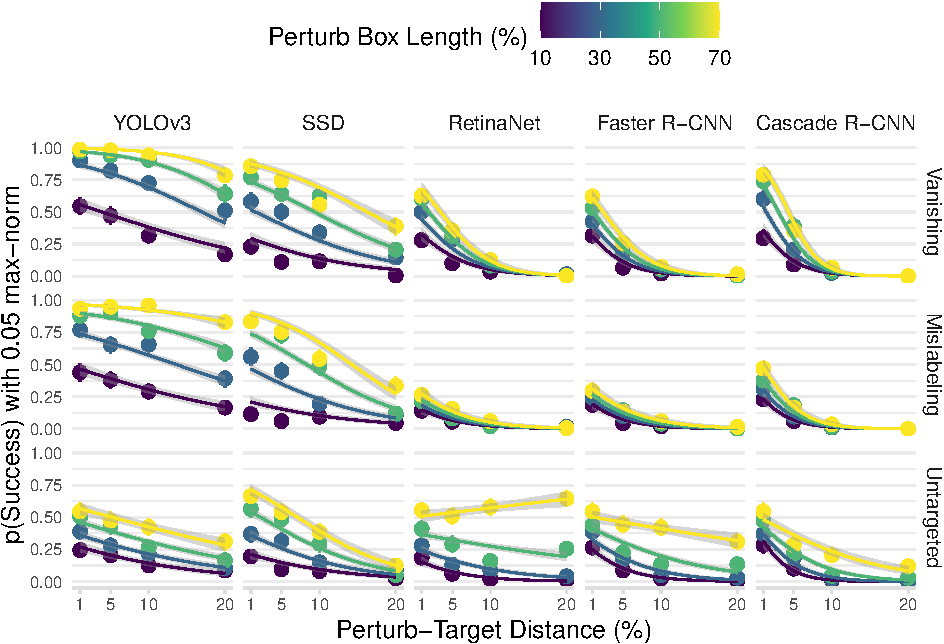
\includegraphics[width=1\linewidth]{imgs-normed/arbitrary_trend_graph-1} 

}

\caption{Perturbing an arbitrary region obfuscates intent with increased success for all models and attacks even with 0.05 max-norm:  We implement intent obfuscating attack by perturbing an arbitrary non-overlapping square region to disrupt a randomly selected target object at various lengths and distances. The binned summaries and regression trendlines graph success proportion against perturb-target distance and perturb box length, both relative to image width or height, in the deliberate attack experiment. Errors are 95\% confidence intervals and every point aggregates success over 200 images. The deliberate attack multiplies success as compared to the randomized attack (Figure \ref{fig:success_trend_graph}), especially at close perturb-target distance and large perturb box length. Full details are given in Section \ref{sec:del_arb}.}\label{fig:arbitrary_trend_graph}
\end{figure}

\begingroup\fontsize{9}{11}\selectfont

\begin{longtable}[t]{llllrrrrrr}
\caption{\label{tab:rand_arb_compare_table}We combined the data in the randomized and deliberate attack experiments to run a logistic model regressing success against object (versus non-object), with perturb-target distance and perturb box size as covariates, both relative to image width or height. The ``object'' term codes object as 1 and non-object as 0. Perturbing an object (in the randomized attack) rather than a non-object (in the deliberate attack) significantly decreases success rates for all model and attack combinations, after controlling for perturb sizes and perturb-target distances. Table headers are explained in Appendix \ref{app:tab_hdr}.}\\
\toprule
\multicolumn{2}{c}{Group} & \multicolumn{8}{c}{Regression} \\
\cmidrule(l{3pt}r{3pt}){1-2} \cmidrule(l{3pt}r{3pt}){3-10}
 & Attack & term & sig & estimate & std.error & statistic & p.value & conf.low & conf.high\\
\midrule
\addlinespace[0.3em]
\multicolumn{10}{l}{\textbf{YOLOv3}}\\
\hspace{1em} & Vanishing & object & * & -0.652 & 0.068 & -9.554 & 0.000 & -0.786 & -0.518\\
\cmidrule{3-10}\nopagebreak
\hspace{1em} &  & distance & * & -8.411 & 0.505 & -16.639 & 0.000 & -9.417 & -7.435\\
\cmidrule{3-10}\nopagebreak
\hspace{1em} &  & size & * & 16.598 & 0.869 & 19.097 & 0.000 & 14.934 & 18.341\\
\cmidrule{3-10}\nopagebreak
\hspace{1em} &  & distance * size & * & -47.808 & 4.879 & -9.798 & 0.000 & -57.511 & -38.378\\
\cmidrule{2-10}\nopagebreak
\hspace{1em} & Mislabeling & object & * & -0.609 & 0.065 & -9.412 & 0.000 & -0.736 & -0.482\\
\cmidrule{3-10}\nopagebreak
\hspace{1em} &  & distance & * & -8.339 & 0.481 & -17.321 & 0.000 & -9.298 & -7.411\\
\cmidrule{3-10}\nopagebreak
\hspace{1em} &  & size & * & 8.671 & 0.501 & 17.299 & 0.000 & 7.708 & 9.674\\
\cmidrule{3-10}\nopagebreak
\hspace{1em} &  & distance * size & * & -10.405 & 3.246 & -3.205 & 0.001 & -16.804 & -4.076\\
\cmidrule{2-10}\nopagebreak
\hspace{1em} & Untargeted & object & * & -0.754 & 0.081 & -9.276 & 0.000 & -0.915 & -0.596\\
\cmidrule{3-10}\nopagebreak
\hspace{1em} &  & distance & * & -11.625 & 0.794 & -14.649 & 0.000 & -13.213 & -10.102\\
\cmidrule{3-10}\nopagebreak
\hspace{1em} &  & size & * & 1.812 & 0.290 & 6.251 & 0.000 & 1.245 & 2.381\\
\cmidrule{3-10}\nopagebreak
\hspace{1em} &  & distance * size & * & 14.484 & 2.744 & 5.278 & 0.000 & 9.123 & 19.884\\
\cmidrule{1-10}\pagebreak[0]
\addlinespace[0.3em]
\multicolumn{10}{l}{\textbf{SSD}}\\
\hspace{1em} & Vanishing & object & * & 0.246 & 0.068 & 3.621 & 0.000 & 0.113 & 0.379\\
\cmidrule{3-10}\nopagebreak
\hspace{1em} &  & distance & * & -14.818 & 0.721 & -20.550 & 0.000 & -16.258 & -13.431\\
\cmidrule{3-10}\nopagebreak
\hspace{1em} &  & size & * & 5.337 & 0.337 & 15.851 & 0.000 & 4.685 & 6.005\\
\cmidrule{3-10}\nopagebreak
\hspace{1em} &  & distance * size &  & 3.676 & 2.807 & 1.309 & 0.190 & -1.832 & 9.177\\
\cmidrule{2-10}\nopagebreak
\hspace{1em} & Mislabeling & object &  & -0.066 & 0.071 & -0.939 & 0.348 & -0.205 & 0.072\\
\cmidrule{3-10}\nopagebreak
\hspace{1em} &  & distance & * & -14.788 & 0.815 & -18.149 & 0.000 & -16.417 & -13.223\\
\cmidrule{3-10}\nopagebreak
\hspace{1em} &  & size & * & 5.484 & 0.333 & 16.489 & 0.000 & 4.839 & 6.143\\
\cmidrule{3-10}\nopagebreak
\hspace{1em} &  & distance * size &  & 0.065 & 2.988 & 0.022 & 0.983 & -5.800 & 5.917\\
\cmidrule{2-10}\nopagebreak
\hspace{1em} & Untargeted & object &  & -0.004 & 0.075 & -0.060 & 0.952 & -0.151 & 0.142\\
\cmidrule{3-10}\nopagebreak
\hspace{1em} &  & distance & * & -15.892 & 0.944 & -16.828 & 0.000 & -17.786 & -14.084\\
\cmidrule{3-10}\nopagebreak
\hspace{1em} &  & size & * & 3.265 & 0.295 & 11.078 & 0.000 & 2.691 & 3.847\\
\cmidrule{3-10}\nopagebreak
\hspace{1em} &  & distance * size &  & 5.899 & 3.236 & 1.823 & 0.068 & -0.458 & 12.233\\
\cmidrule{1-10}\pagebreak[0]
\addlinespace[0.3em]
\multicolumn{10}{l}{\textbf{RetinaNet}}\\
\hspace{1em} & Vanishing & object & * & -0.500 & 0.092 & -5.453 & 0.000 & -0.681 & -0.321\\
\cmidrule{3-10}\nopagebreak
\hspace{1em} &  & distance & * & -28.569 & 1.820 & -15.698 & 0.000 & -32.231 & -25.097\\
\cmidrule{3-10}\nopagebreak
\hspace{1em} &  & size & * & 2.814 & 0.351 & 8.006 & 0.000 & 2.130 & 3.509\\
\cmidrule{3-10}\nopagebreak
\hspace{1em} &  & distance * size &  & 4.598 & 6.024 & 0.763 & 0.445 & -7.315 & 16.315\\
\cmidrule{2-10}\nopagebreak
\hspace{1em} & Mislabeling & object & * & -0.444 & 0.130 & -3.413 & 0.001 & -0.703 & -0.192\\
\cmidrule{3-10}\nopagebreak
\hspace{1em} &  & distance & * & -30.944 & 2.839 & -10.901 & 0.000 & -36.733 & -25.604\\
\cmidrule{3-10}\nopagebreak
\hspace{1em} &  & size & * & 0.990 & 0.434 & 2.282 & 0.022 & 0.141 & 1.842\\
\cmidrule{3-10}\nopagebreak
\hspace{1em} &  & distance * size & * & 19.990 & 8.749 & 2.285 & 0.022 & 2.681 & 37.028\\
\cmidrule{2-10}\nopagebreak
\hspace{1em} & Untargeted & object & * & -0.337 & 0.085 & -3.972 & 0.000 & -0.504 & -0.171\\
\cmidrule{3-10}\nopagebreak
\hspace{1em} &  & distance & * & -14.091 & 1.029 & -13.692 & 0.000 & -16.158 & -12.124\\
\cmidrule{3-10}\nopagebreak
\hspace{1em} &  & size & * & 3.062 & 0.300 & 10.202 & 0.000 & 2.475 & 3.652\\
\cmidrule{3-10}\nopagebreak
\hspace{1em} &  & distance * size & * & 32.836 & 3.065 & 10.714 & 0.000 & 26.912 & 38.930\\
\cmidrule{1-10}\pagebreak[0]
\addlinespace[0.3em]
\multicolumn{10}{l}{\textbf{Faster R-CNN}}\\
\hspace{1em} & Vanishing & object & * & -1.017 & 0.117 & -8.659 & 0.000 & -1.250 & -0.790\\
\cmidrule{3-10}\nopagebreak
\hspace{1em} &  & distance & * & -27.903 & 2.147 & -12.997 & 0.000 & -32.247 & -23.831\\
\cmidrule{3-10}\nopagebreak
\hspace{1em} &  & size & * & 2.870 & 0.392 & 7.320 & 0.000 & 2.107 & 3.644\\
\cmidrule{3-10}\nopagebreak
\hspace{1em} &  & distance * size &  & -13.406 & 7.814 & -1.716 & 0.086 & -28.896 & 1.751\\
\cmidrule{2-10}\nopagebreak
\hspace{1em} & Mislabeling & object & * & -0.999 & 0.146 & -6.866 & 0.000 & -1.291 & -0.720\\
\cmidrule{3-10}\nopagebreak
\hspace{1em} &  & distance & * & -23.220 & 2.264 & -10.254 & 0.000 & -27.839 & -18.962\\
\cmidrule{3-10}\nopagebreak
\hspace{1em} &  & size & * & 1.062 & 0.426 & 2.490 & 0.013 & 0.225 & 1.897\\
\cmidrule{3-10}\nopagebreak
\hspace{1em} &  & distance * size &  & 2.781 & 7.934 & 0.350 & 0.726 & -13.013 & 18.122\\
\cmidrule{2-10}\nopagebreak
\hspace{1em} & Untargeted & object & * & -0.497 & 0.093 & -5.319 & 0.000 & -0.682 & -0.315\\
\cmidrule{3-10}\nopagebreak
\hspace{1em} &  & distance & * & -18.743 & 1.235 & -15.173 & 0.000 & -21.226 & -16.383\\
\cmidrule{3-10}\nopagebreak
\hspace{1em} &  & size & * & 1.824 & 0.308 & 5.925 & 0.000 & 1.222 & 2.429\\
\cmidrule{3-10}\nopagebreak
\hspace{1em} &  & distance * size & * & 35.146 & 3.351 & 10.487 & 0.000 & 28.643 & 41.785\\
\cmidrule{1-10}\pagebreak[0]
\addlinespace[0.3em]
\multicolumn{10}{l}{\textbf{Cascade R-CNN}}\\
\hspace{1em} & Vanishing & object & * & -0.921 & 0.105 & -8.773 & 0.000 & -1.128 & -0.717\\
\cmidrule{3-10}\nopagebreak
\hspace{1em} &  & distance & * & -35.343 & 2.414 & -14.641 & 0.000 & -40.213 & -30.751\\
\cmidrule{3-10}\nopagebreak
\hspace{1em} &  & size & * & 5.069 & 0.428 & 11.831 & 0.000 & 4.242 & 5.923\\
\cmidrule{3-10}\nopagebreak
\hspace{1em} &  & distance * size & * & -37.908 & 9.338 & -4.060 & 0.000 & -56.487 & -19.857\\
\cmidrule{2-10}\nopagebreak
\hspace{1em} & Mislabeling & object & * & -0.851 & 0.127 & -6.708 & 0.000 & -1.103 & -0.605\\
\cmidrule{3-10}\nopagebreak
\hspace{1em} &  & distance & * & -32.428 & 2.950 & -10.994 & 0.000 & -38.452 & -26.886\\
\cmidrule{3-10}\nopagebreak
\hspace{1em} &  & size & * & 2.849 & 0.398 & 7.151 & 0.000 & 2.071 & 3.633\\
\cmidrule{3-10}\nopagebreak
\hspace{1em} &  & distance * size &  & -14.661 & 10.223 & -1.434 & 0.152 & -34.890 & 5.215\\
\cmidrule{2-10}\nopagebreak
\hspace{1em} & Untargeted & object & * & -0.615 & 0.101 & -6.082 & 0.000 & -0.815 & -0.419\\
\cmidrule{3-10}\nopagebreak
\hspace{1em} &  & distance & * & -29.517 & 1.920 & -15.376 & 0.000 & -33.393 & -25.864\\
\cmidrule{3-10}\nopagebreak
\hspace{1em} &  & size & * & 1.311 & 0.322 & 4.077 & 0.000 & 0.682 & 1.943\\
\cmidrule{3-10}\nopagebreak
\hspace{1em} &  & distance * size & * & 33.612 & 5.105 & 6.584 & 0.000 & 23.655 & 43.689\\
\bottomrule
\end{longtable}
\endgroup{}

\end{document}
